% !TEX root = ../main.tex

%%%%%%%%%%%%%%%%%%%%%%%%%%%%%%%%%%%%%%%%%%%%%%%%%%%%%%%%%%%%%%%%%%%%%%%%%%%%
% 第五章：实验评估
%%%%%%%%%%%%%%%%%%%%%%%%%%%%%%%%%%%%%%%%%%%%%%%%%%%%%%%%%%%%%%%%%%%%%%%%%%%%
\chapter{实验评估和现象分析}
\label{ch:evaluation}

\section{实验设置}
本章通过端到端请求重放实验，比较基于性能预测的调度策略与开源社区、学术界和工业界代表性策略在LLM推理服务中的性能表现，从而评估本文所提出性能预测模块对调度决策的实际收益。

\subsection{对比策略}
为展示简单负载指标混合方法的局限性，本文选取了若干基于实例当前指标组合进行决策的代表性策略，并将其与本文实现的预测驱动策略进行比较。
为了排除系统实现和框架差异对结果的干扰，所有策略都在统一的Rust全局调度框架上实现。该框架已经过性能校准，以保证不同策略在相同系统条件下进行公平比较。同时，本文也对各策略的实现进行了语义校验，确保其行为与原始设计保持一致。具体比较对象如下：

\begin{itemize}
  \item \textbf{Company-X}：工业界在线上环境使用的代表性策略，通过线性组合多个实例指标形成调度得分。为展示其最优效果，本文对每个工作负载分别进行了参数调优。
  \item \textbf{vLLM}：开源推理服务中广泛使用的策略，采用基于等待请求数和运行请求数混合的负载均衡方法。
  \item \textbf{Dynamo}：NVIDIA 公布的推理框架中使用的策略，采用Prefill Token数和实例总Token数的线性组合来刻画实例负载。本文同样对其组合参数进行了调优。
  \item \textbf{Predictor}：本文实现的预测驱动策略。调度器调用在线性能预测模块，估计请求在各实例上完成Prefill的时延，并将请求指派到预测TTFT最小的实例。
\end{itemize}

\subsection{硬件与部署环境}
实验平台为一台配备8张 NVIDIA H20 的 DGX 节点，每张 GPU 具有 96GB 显存。全局调度器、请求重放工具和所有模型实例部署在一台拥有 176 个 Intel Xeon CPU 核心和 1TB DRAM 的服务器上。
对于模型部署与推理执行，本文选用 vLLM-v1 作为推理引擎，并使用 FlashInfer 作为 Attention 后端。
实验采用PD共置方式部署实例，每张GPU部署一个模型实例，因此共构成8实例的推理服务集群，用于端到端请求重放。

\subsection{模型与工作负载}
为验证本文方法在不同模型架构下的适用性，实验选取了两类结构差异较大的模型：
\begin{itemize}
  \item \textbf{Qwen2.5-7B}：Dense 架构模型；
  \item \textbf{Qwen3-30B-A3B}：MoE 架构模型。
\end{itemize}

工作负载方面，本文使用多种开源请求轨迹进行重放，覆盖不同LLM应用场景：
\begin{itemize}
  \item \textbf{Qwen ChatBot}：来自通用对话场景；
  \item \textbf{Qwen Coder}：来自代码补全与辅助编程场景；
  \item \textbf{Qwen Agent}：来自智能体调用场景；
  \item \textbf{ToolAgent (Kimi)}：来自工具调用较频繁的Agent服务场景。
\end{itemize}

\subsection{请求重放方法}
由于原始工作负载的采集环境与本文测试环境在集群规模、模型部署和推理框架上均存在差异，原始请求到达速率不能直接用于当前实验平台。
因此，本文使用开源请求重放器 Trace-Replayer 对原始时间戳进行缩放，以构造适配当前系统服务能力的负载强度。
具体而言，本文通过比较不同缩放比例下系统的 Mean TTFT、Mean TPOT 及 SLO 违反请求数，选取处于系统服务能力区间内的多个代表性负载点，并在这些负载点上对不同策略进行端到端性能对比。


\section{端到端性能结果分析}
\label{sec:e2e_results}

\begin{figure}[t]
\centering
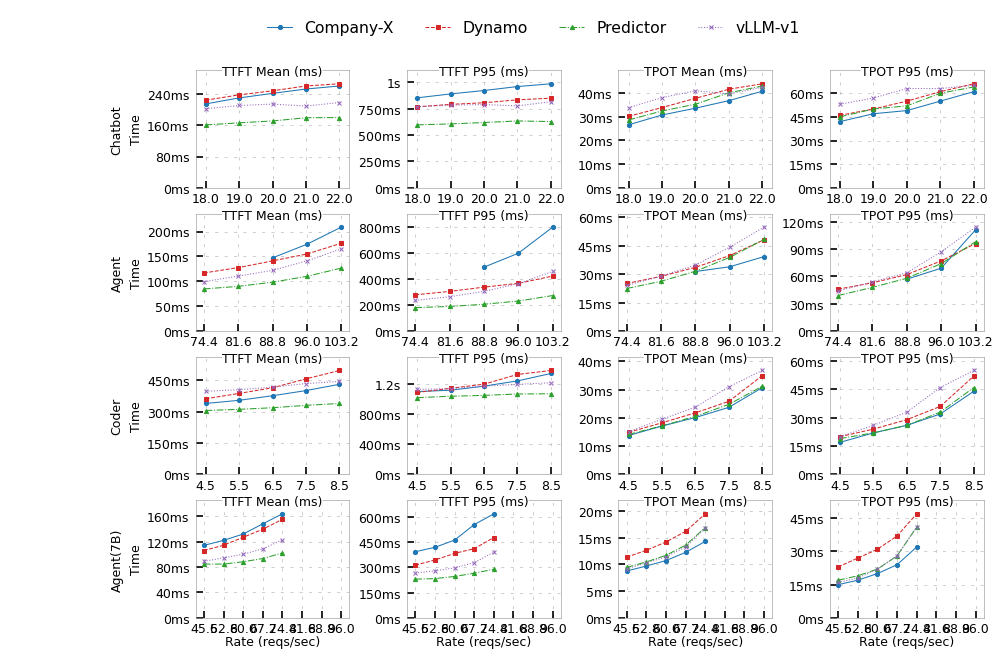
\includegraphics[width=0.9\textwidth]{figures/e2e/e2e_new_fig.png}
\caption{部署Qwen3-30B-A3B模型在不同工作负载和请求到达速率下，性能预测策略与基线策略在TTFT Mean, TTFT P95, TPOT Mean和TPOT P95性能指标上的性能对比}
\label{fig:e2e_comparison}
\end{figure}

图~\ref{fig:e2e_comparison}展示了在各工作负载服务能力区间内，不同策略在TTFT和TPOT（mean/p95）指标上的对比结果。
总体上，基于TTFT预测的调度策略在所有场景下均能够明显改善TTFT。例如，在Qwen ChatBot负载、22 QPS下，相比Company-X策略能够带来31.0\%的TTFT Mean提升和36.3\%的TTFT P95提升；相比vLLM-v1策略，则在Qwen Coder负载、7.5 QPS下带来24.0\%的TTFT Mean提升和10.7\%的TTFT P95提升。
更重要的是，这种TTFT收益并未以显著恶化TPOT为代价。与TPOT表现最优或接近最优的Company-X相比，Predictor在Qwen Coder负载、7.5 QPS下仅带来4.4\%的TPOT Mean下降和3.1\%的TPOT P95下降，但整体表现仍明显优于Dynamo和vLLM。
这表明，基于TTFT性能预测模块的调度策略不仅能够显著降低首token时延，还能够在一定程度上兼顾流式生成阶段的性能表现。

造成这一结果的原因在于，本文预测的并非单一负载指标，而是请求在当前实例状态下的实际执行时长。该预测过程中已经隐式综合了Token数、Decode请求数、KVCache大小等多种影响因素。
因此，Predictor实际上将原本需要人工组合和调参的多维负载信息统一映射为一个直接面向服务目标的调度得分。与显式组合少量基础指标相比，这种方式能够更加完整地利用实例状态信息，并在TPOT变化有限的前提下取得更稳定的TTFT收益。



\section{预测准确性分析}
% \begin{figure}[t]
% \centering
% \includegraphics[width=0.9\textwidth]{figures/accuracy/prediction_error.png}
% \caption{Qwen2.5-7B和Qwen3-30B-A3B模型预测TTFT与真实TTFT误差CDF对比}
% \label{fig:pred_accuracy}
% \end{figure}
本节分析本文实现的性能预测模块能否对请求在目标实例上的TTFT给出足够准确的估计。
严格来说，在线调度场景中的理想评估应比较“每个时刻、每个候选实例上的反事实TTFT”与真实执行结果；但在真实系统中，我们无法同时观察所有这些反事实结果。
因此，本文采用一种可操作的近似评估方式：对于请求 \(i\)，记录性能预测模块给出的各实例预测值 \(\text{Pred}_i\)；当请求被实际指派到实例 \(j\) 后，再记录该实例上的真实TTFT \(\text{Real}_i\)。随后从 \(\text{Pred}_i\) 中取出对应实例 \(j\) 的预测结果，并与 \(\text{Real}_i\) 比较，从而得到该请求在真实指派实例上的预测误差。

通过对一次端到端请求重放中的全部请求执行上述统计，可以得到预测误差的CDF曲线，从整体上观察预测模块的误差分布。
具体而言，本文分别在Qwen2.5-7B和Qwen3-30B-A3B模型上，于(TODO!)工作负载的(TODO!)和(TODO!)请求到达速率下记录所有 \(\text{TTFT(Real)}_i\) 与 \(\text{TTFT(Pred)}_{i,j}\)，并绘制误差CDF，如(TODO!)所示。
结果表明，在Qwen2.5-7B对应的执行环境中，预测误差整体较小，(TODO!)的请求误差位于(TODO!)以内；而在MoE架构的Qwen3-30B-A3B模型上，预测误差相对更大，但仍有(TODO!)的请求误差位于(TODO!)以内。

\section{跨表迁移现象分析}
\label{sec:crosstable}

% \begin{figure}[t]
% \centering
% \includegraphics[width=0.9\textwidth]{fig/accuracy/cross_table_e2e.png}
% \caption{Qwen3-30B-A3B模型下正常预测与跨表预测（使用Qwen2.5-7B预测表）的端到端测试TTFT/TPOT对比}
% \label{fig:crosstable_perf}
% \end{figure}
当部署模型大小或硬件资源配置发生变化时，模拟器通常需要重新进行离线性能剖析并生成新的预测表。对于同时服务大量模型、且部署环境多样的LLM服务厂商而言，这意味着较高的适配与维护成本。
不过，不同模型在结构上通常仍具有一定相似性，例如都包含Attention和MLP（或MoE）等组件，影响执行时间的因素也大体一致，只是预测表中具体的时间映射系数不同。
对于离线模拟而言，模拟器的目标是支持集群吞吐分析和容量规划，因此需要尽可能准确地预测绝对执行时间；但在调度场景中，预测值主要用于比较候选实例并选出目标实例，只要能够较好反映不同实例之间的相对负载即可。
基于上述两个原因，在在线场景中不同模型的预测表可能存在迁移、复用的可能性，即使用与模型部署不同配置的性能预测表来指导调度决策。

本小节尝试在端到端测试中使用与部署模型不同的预测表来指导调度决策，并分析这种跨表迁移是否可行。如图(TODO!)所示，本文在(TODO!)工作负载中部署Qwen3-30B-A3B，并在全局调度器中使用Qwen2.5-7B模型的预测表进行性能预测（后续称为跨表预测），再比较端到端请求重放中的TTFT与TPOT。
实验结果表明，跨表迁移部署的TTFT Mean与正常部署相比仅低(TODO!)，TPOT Mean仅低(TODO!)。虽然TTFT P99和TPOT P99的差距更大，但整体退化仍然有限；同时，相比Company-X策略，跨表迁移后的TTFT Mean仍有(TODO!)的性能提升，而TPOT Mean仅慢(TODO!)。
这意味着，即使模型架构存在差异（Dense与MoE），跨表迁移带来的端到端性能下降仍然相对有限，并且相较于简单指标混合策略，仍能保持明显的TTFT优势。


\subsection{Spearman 秩相关与选择一致率}
\label{sec:spearman}

在这一小节中，本文进一步分析上述跨表迁移现象产生的原因。具体而言，在同一次请求重放测试中，同时使用跨表预测的模拟器和正确配置的模拟器进行性能预测；对于每个请求 $r$，记录候选实例集合 $\mathcal{I}$ 上两张预测表输出的性能指标 $\{TTFT_A(r,i)\}$ 与 $\{TTFT_B(r,i)\}$。
随后将评分转为排序，计算两者的Spearman相关系数 $\rho(r)$，并统计全体请求的平均值和分位数（TODO: 公式可简述）。
同时，本文还计算两张预测表的 Top-1 选择一致率，即两张预测表是否为同一请求选择了相同的最优实例。

在对(TODO!)工作负载的请求重放中发现，虽然两张预测表在绝对TTFT数值上存在一定偏移，但它们对候选实例的相对排序通常仍保持较高一致性。
这说明跨表迁移之所以能够在端到端实验中取得可接受的效果，关键并不在于预测绝对值完全准确，而在于其仍能较好保留不同实例之间的优劣顺序。
换言之，在线调度真正依赖的是排序信息而非绝对时长；只要排序稳定，跨表迁移就仍然具有实用价值。
\section{在线开销与可扩展性分析}
\label{sec:online_budget}

% \begin{figure}[t]
% \centering
% \includegraphics[width=0.9\textwidth]{fig/scale/scalability.png}
% \caption{可扩展性测试中性能预测模块吞吐与集群服务能力随实例数扩展的对比（使用ChatBot工作负载）}
% \label{fig:scalability}
% \end{figure}
在调度场景中引入性能预测模块后，相比直接混合少量基础指标，系统实现逻辑更为复杂，因此一个关键问题是：该模块是否能够支撑更大规模集群下的在线调度需求。
本节通过压力测试估计预测模块在不同实例规模下的吞吐上界，并将其与系统服务能力的扩展趋势进行对比，从而分析预测模块是否会先于系统本身成为瓶颈。
由于硬件资源限制，我们无法在真实的8实例以上规模集群下进行测试。因此，为了扩展集群规模，本文让每个物理实例在全局调度器中对应多个逻辑实例，且这些逻辑实例状态与物理实例完全同步。对全局调度器而言，这可以近似视作在更大规模集群上进行调度。
在压力测试中，请求发送器持续向全局调度器发送请求。为避免推理实例被超载请求压垮，本文限制每个逻辑实例可承载的Token总数；如果新到达请求会使逻辑实例Token数超出上限，则在调度结束后拒绝该次请求指派。
通过这一方式，本文在无法继续扩展物理硬件规模的情况下，近似评估了更大规模集群下的调度吞吐压力。集群服务能力方面，本文以(TODO!)负载在8实例下满足TTFT P99和TPOT P99 SLO约束时的QPS作为8实例集群的服务能力上界，并假设在合理调度下集群吞吐随实例数近似线性扩展，由此推导不同实例数下的系统服务能力上界。
随后将预测模块吞吐与该服务能力上界进行对比，以得到可扩展性分析结果。

总体结果显示，本文的在线模拟器在(TODO!)负载下，即使扩展到(TODO!)实例规模，仍然能够支撑在线服务，不会成为系统瓶颈。

\section{本章小结}
本章在8卡NVIDIA H20集群上，使用Qwen2.5-7B和Qwen3-30B-A3B两种模型，覆盖ChatBot、Coder、Agent和ToolAgent四类工作负载，从四个维度对基于性能预测的调度策略进行了系统评估。
端到端性能对比表明，预测驱动的策略在所有场景下均显著降低TTFT，且未以大幅牺牲TPOT为代价。
预测准确性分析验证了模拟器对Dense模型具有较高的预测精度，MoE模型因专家路由动态性误差略大。
跨表迁移实验发现，使用不同模型的预测表指导调度仍能保持较高的决策一致率和相近的端到端性能，为快速适配新模型提供了可行路径。
可扩展性测试表明，预测模块的吞吐在64实例规模下仍高于集群服务能力上界，验证了其在大规模部署中的在线可用性。
